\chapter{Lighthouse Taxonomy}
\label{lighthousechap}

Lighthouse is a web application designed for helping scientists, engineers, students and linear algebra enthusiasts with the implementation of the high-performance matrix algebra computations. Like a lighthouse that helps sailors navigate their ships in the dark seas, Lighthouse guides the numerical linear algebra practitioners through the dark seas of numerical software development. It is the first framework that attempts to combine a matrix algebra software ontology with code generation and tuning capabilities. Lighthouse will offer all of the software needed to take a linear algebra problem from its algorithmic description to a high-performance implementation.

Section 3.1 of this chapter describes the existing taxonomies and their shortcomings. Section 3.2 explains the main objectives of Lighthouse. Section 3.3 describes the LAPACK routine search engine that has been partially implemented followed by Section 3.4 covering the different user interfaces that Lighthouse currently has. Section 3.5 talks about the tuning tool Lighthouse uses for automatic code optimization. Section 3.6 discusses my personal contribution to the development of Lighthouse.

\section{Existing taxonomies}
There are some numerical software taxonomies that let users find stand-alone algorithms, download codes, compile, optimize or use the code through a domain-specific web interface. Netlib \cite{netlib} and GAMS \cite{gams} offer extensive collections of numerical software but it is not always easy to find the right files or routines using the searching service they provide. For example, on Netlib, a simple keyword search ``solve linear system'' can return routines for solving various matrix algebra problems, conference papers, documentation files, and broken links. Moreover, these taxonomies do not provide enough information about the right routines or files they do return. GAMS provides a single sentence or partial sentence for each piece of software it returns, which is rarely enough. Netlib's search results vary widely in detail. Some items contain just the file name whereas some items contain a lot of information. The LAPACK Search Engine \cite{lapacksearch} provides help with various LAPACK-related language but in the end delivers only the code but no additional information regarding how to use it.

These taxonomies use function level indexing, which is categorizing the routines contained in the libraries based on their functionalities. This technique, however, cannot accommodate high-level operations for which no library implementation is available or for which complex software packages such as PETSc \cite{petsc} or Trilinos \cite{trilinos} are required. As a result, it can be very challenging or impossible to represent and maintain the functionality of large toolkits, such as PETSc, in existing taxonomies.

\section{The main goals of Lighthouse}
Lighthouse attempts to address three main challenges of numerical linear algebra computations. First, a huge amount of software is available for numerical linear algebra computation and finding the appropriate software for solving a particular problem can be quite difficult. Lighthouse provides a collection of the most widely used software and a user-friendly web interface to find the suitable software for solving various linear algebra problems. Second, writing matrix algebra code in general is not easy for individuals without computer science backgrounds. Lighthouse offers a code generation service for producing code from the algorithmic description of a linear algebra problem. And third, optimizing matrix algebra code is a daunting task and optimization is absolutely necessary for producing high-performance code. It requires expertise in compiler construction, code optimization, and computer architecture. Lighthouse provides an optimization facility to help users create high-performance matrix algebra code. Our target is to make the Lighthouse taxonomy easy to use and to provide enough information about all routines included in the taxonomy so that a computational scientist seeking to build a good implementation will understand what the various parts entail.

\section{Lighthouse for LAPACK}
The development of Lighthouse was inspired by the potential of the LAPACK Search Engine \cite{lapacksearch}. LAPACK (Linear Algebra PAckage) is a software package written in Fortran 90. It provides routines for solving the most important numerical linear algebra problems, that is, solving systems of linear equations, least-square solutions of linear systems of equations, eigenvalue and singular value problems. It also provides routines for various matrix factorization methods such as LU decomposition, Cholesky and QR facrozation, Schur and generalized Schur factorization. In addition, LAPACK also offers routines for reordering Schur factorization and estimating condition numbers of matrices. It can handle dense and banded matrices, however it does not provide support for handling sparse matrices. It can also handle real and complex numbered matrices in both single and double precision. All the routines rely on the Basic Linear Algebra Subprograms (BLAS) which is the de facto support routine package for performing basic level linear algebra operations. LAPACK tries to exploit the level 3 BLAS, which are routines for doing various matrix multiplication and solving triangular systems of linear equations. Since the Level 3 BLAS routines loosely coupled, using these routines promotes high efficiency on many high-performance computers. If these routines are provided by the hardware manufacturer, the efficiency of these routines can be very high.  

The Lighthouse taxonomy is continuously expanding and currently includes over a thousand LAPACK subroutines. The taxonomic information is stored in a relational database. First, the subroutines are grouped by the types of tasks they perform. The system then sorts and identifies eleven different matrix types based on five different storage properties. Then it categorizes the subroutines based on whether they handle single or double precision numbers and real or complex numbers. This allows very fast searching of the routines based on any combination of task, matrix type, storage format, precision level and number type.

Lighthouse is developed using some of the most popular open-source tools currently available. The main infrastructure of Lighthouse is built on the Django framework \cite{django}, an open source high-level Python Web framework. Django provides a dynamic database access application programming interface (API) and supports an automatic administrative interface that makes future data maintenance simple and convenient. For storing the taxonomic information, Lighthouse uses a MySQL \cite{mysql} database, the world's most widely used open source database management system. In addition, Lighthouse uses Haystack \cite{haystack}, a modular search application for Django that offers powerful database queries and multiple search indices. For additional functionalities, Lighthouse uses a JavaScript toolkit called Dojo \cite{dojo}. Dojo is an open source modular JavaScript library designed to aid rapid development of cross-platform, JavaScript/Ajax-based applications and web sites. AJAX is a collection of interrelated web development techniques used on the client-side to create asynchronous web applications. To ease the process of integrating Dojo into the main Django project, a reusable Django application called Dojango \cite{dojango} is used. Lighthouse uses two other open source Django applications, dajax and dajaxice \cite{dajax}, for fast and easy implementation of AJAX (Asynchronous JavaScript and XML). Figure 3.1 shows the software tools used for building the Lighthouse.

\begin{figure}[h!]\label{lighthousetools}
  \centering
  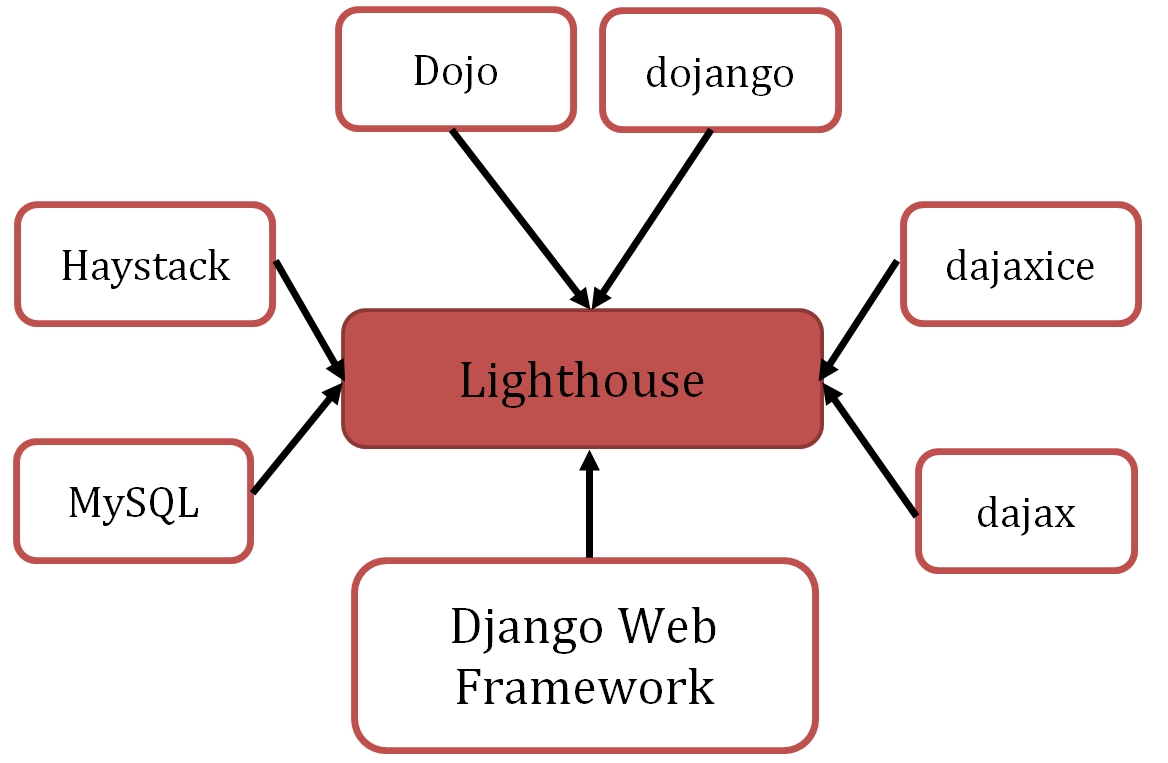
\includegraphics[width=5in]{figs/lighthousetools}
  \caption[Tools used for making Lighthouse]
   {Lighthouse is built with powerful open-source tools, such as Django, MySQL, and Dojo.}
\end{figure}

\section{User interfaces}
Lighthouse provides three different graphical user interfaces to help users of different backgrounds to use the numerical software. Each interface offers the code generation service and tuning tools included in the taxonomy. The following subsections discuss more on the components of the Lighthouse user interfaces.

\subsection{Simple search}
The Simple Search interface guides the users through a series of increasingly detailed questions describing the problems they wish to solve. New questions are automatically generated based on the responses to the earlier questions. Figure 3.2 shows the beginning of a simple search.

\begin{figure}[h!]\label{simplesearch1}
  \centering
  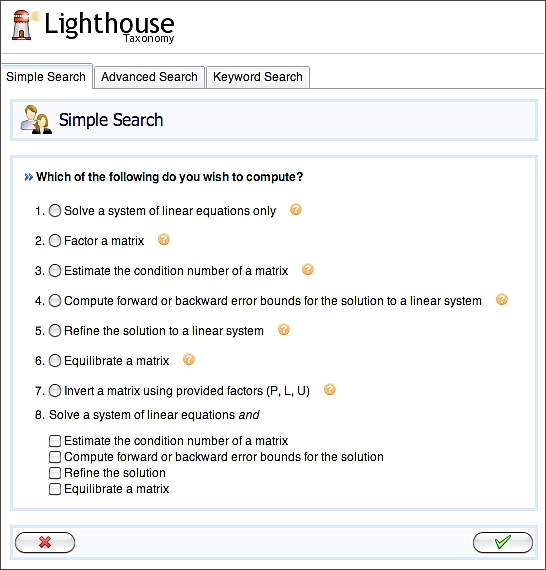
\includegraphics[width=5in]{figs/simplesearch1}
  \caption[Beginning of a simple search]
   {Beginning of a simple search.}
\end{figure}

\noindent After the user chooses what they want to compute (Figure 3.2) Lighthouse generates more detailed questions as shown in Figure 3.3, where three questions have been answered and the next question is being asked. Once the user has answered all the questions, Lighthouse returns a single routine in the search result area of the interface.

\begin{figure}[h!]\label{simplesearch2}
  \centering
  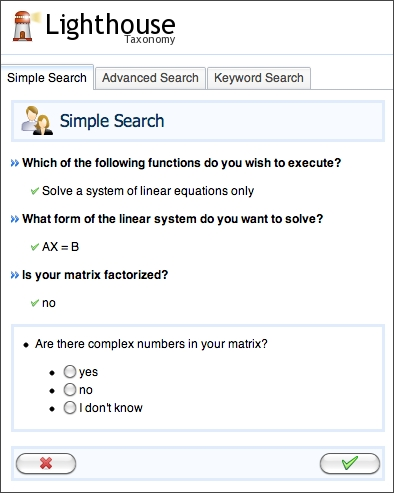
\includegraphics[width=4in]{figs/simplesearch2}
  \caption[A simple search in its mid-stage]
   {A simple search in its mid-stage.}
\end{figure}

 \begin{figure}[h!]\label{simplesearch3}
  \centering
  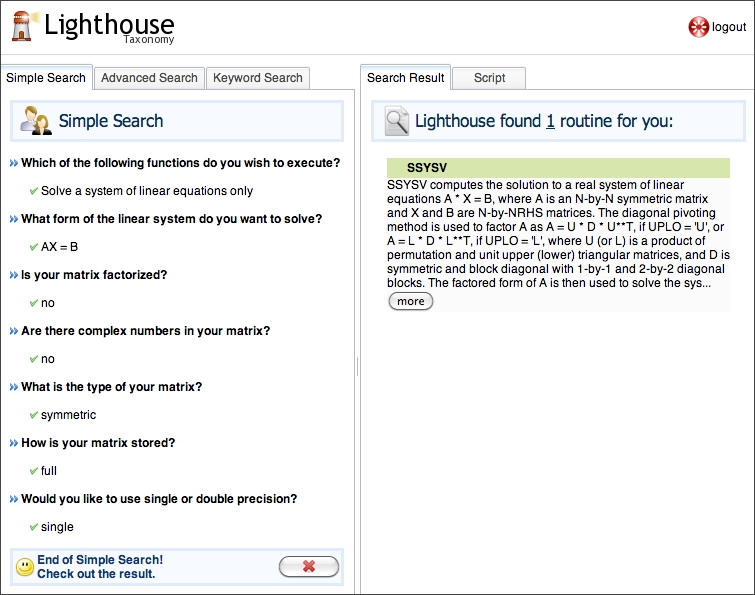
\includegraphics[width=5in]{figs/simplesearch3}
  \caption[The result of a simple search]
   {The result of a simple search.}
\end{figure}

Figure 3.4 shows all the questions answered on the left part of the interface and the routine Lighthouse found on the result area on the right. Information about the questions can be accessed via help buttons located next to the questions allowing users to learn about various numerical linear algebra terms and concepts. Figure 3.5 illustrates the use of help buttons that appear next the questions in a simple search.

\begin{figure}[h!]\label{simplesearch4}
  \centering
  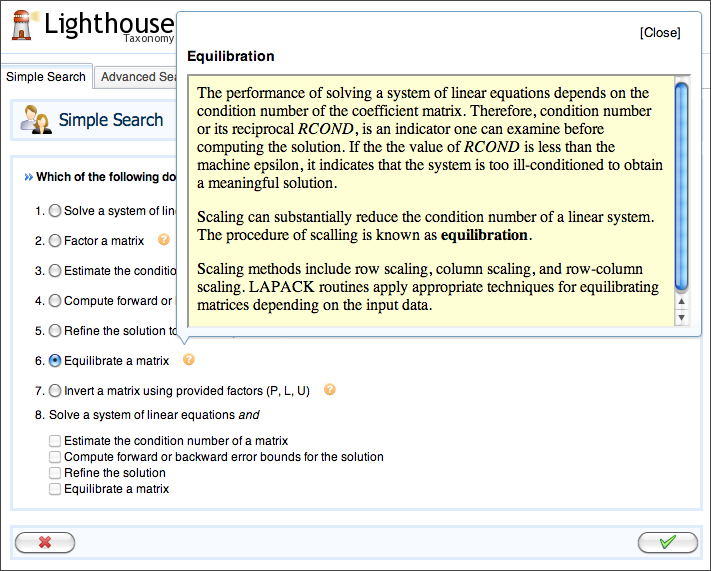
\includegraphics[width=5in]{figs/simplesearch4}
  \caption[Help content about the task ``equilibrate a matrix'']
   {Help content about the task “Equilibrate a matrix”.}
\end{figure}

\subsection{Advanced Search}
The Advanced Search interface has been designed specifically for users who are familiar with LAPACK. First it asks the user what type of routines they would like to search for. Figure 3.6 shows the first step of advanced search.

\begin{figure}[h!]\label{advancedsearch1}
  \centering
  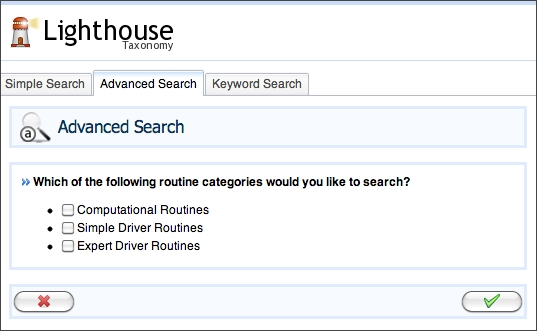
\includegraphics[width=5in]{figs/advancedsearch1}
  \caption[First step of Advanced Search]
   {First step of Advanced Search.}
\end{figure}

After the user selects which type of routines they are looking for (Figure 3.6), Lighthouse then provides a form containing various options that the user can select (Figure 3.7) and Lighthouse will return all the routines that fit the specified options in the search result area. Then the user can pick the routines they think are appropriate for solving the problem at hand or simply search again with different options.

\begin{figure}[h!]\label{advancedsearch2}
  \centering
  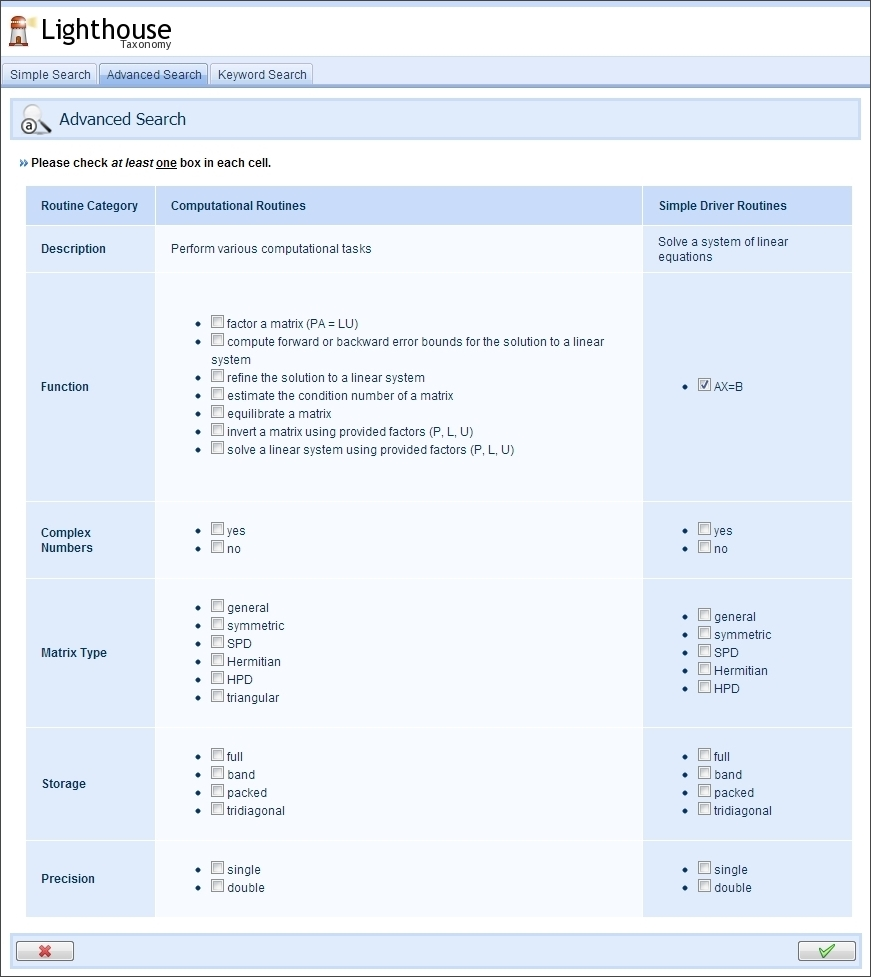
\includegraphics[width=6.5in]{figs/advancedsearch2}
  \caption[Various options in an advanced search]
   {Various options in an advanced search.}
\end{figure}

\subsection{Keyword search}

The Keyword Search interface is much simpler than the other interfaces. It works in a similar way as Netlib's keyword search does. The user has to enter keywords such as ``solve linear systems'' or ``condition number'', the system will return all the subroutines that contain those words in their documentation. The user can then read more information about the routines returned by the search and keep the ones they think are useful. The keyword search interface is shown in Figure 3.8.

\begin{figure}[h!]\label{keywordsearch1}
  \centering
  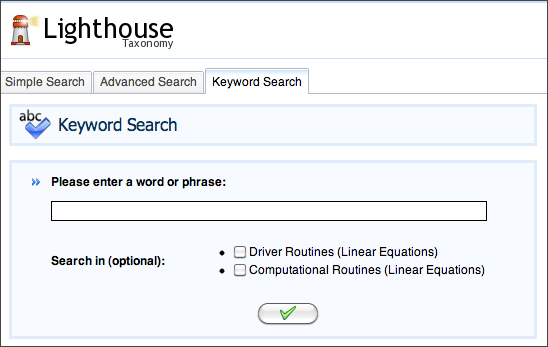
\includegraphics[width=6in]{figs/keywordsearch1}
  \caption[Keyword Search interface]
   {Keyword Search interface.}
\end{figure}

\section{Build to Order (BTO) BLAS System}

Lighthouse uses the Build to Order (BTO) \cite{bto} BLAS System for automatic code tuning. The Build to Order BLAS system is a compiler that generates high-performance implementations of basic linear algebra kernels.
 
The BLAS is a standard API for performing vector-vector, matrix-vector, and matrix-matrix operations. Traditionally, each routine in the BLAS has been implemented manually by hand by a highly skilled programmer. The Build to Order BLAS compiler automates the implementation of the BLAS standard as well as any sequence of basic linear algebra operations. 

The user of the Build to Order BLAS compiler writes down a specification for a sequence of matrix and vector operations together with a description of the input and output parameters. The compiler then tries out many different choices of how to implement, optimize, and tune those operations for the user's computer hardware. The compiler chooses the best option, which is output as a C file that implements the specified operations. 

Under the script tab of the Lighthouse interface, users can write their computation in a high-level MATLAB-like syntax. Then, by interfacing with BTO compiler, Lighthouse generates optimized C implementations of the input script. The users are then able to download the code, modify it, and integrate it into the larger application context. Figure 3.9 illustrates the Lighthouse interface for tuning code.

\begin{figure}[h!]\label{bto}
  \centering
  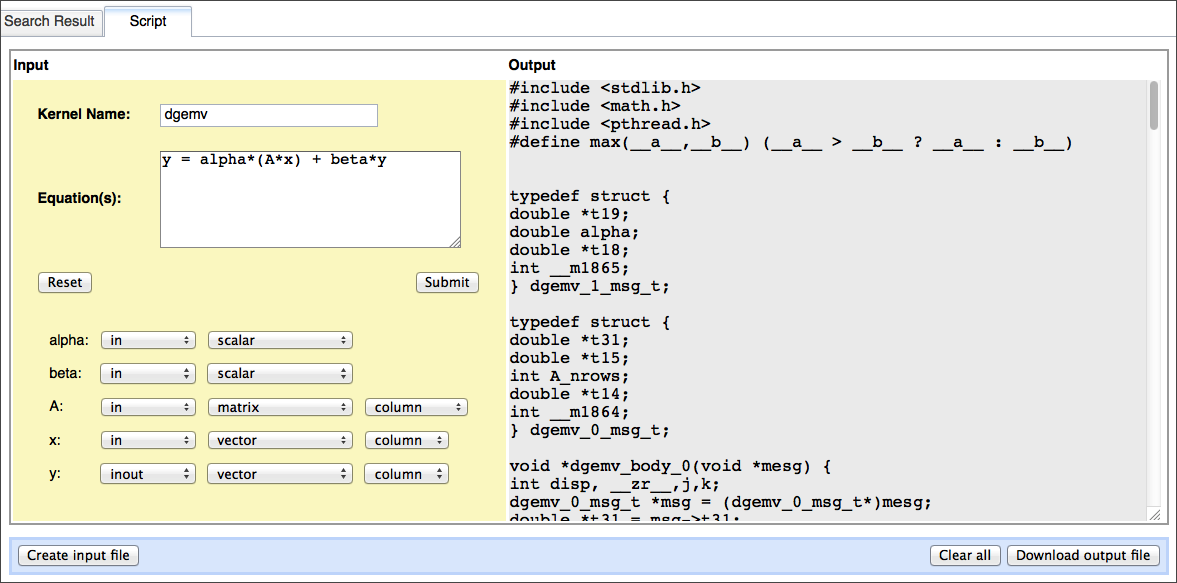
\includegraphics[width=6in]{figs/bto}
  \caption[Build to Order BLAS system]
   {Lighthouse interface for tuning code using the BTO system.}
\end{figure}

\section{My Contributions to Lighthouse}
I joined the Lighthouse team on March 21, 2012. I spent slightly over a month learning Django and getting familiar with Lighthouse and its major components. For the next couple of months (May - June 2012) I designed and added many icons to various parts of Lighthouse and updated the CSS and HTML for enhancing the overall look of the user interfaces. In July and August, I mostly worked with JavaScript and AJAX to improve the client-side interactions such as form validation, added drag and drop functionality for the Advanced Search, updated the session management part of selected routines and implemented routine reordering which allows the user to change the order of the selected routines in the work area. The routine reordering pane is shown in Figure 3.10.

\begin{figure}[h!]\label{routineordering}
  \centering
  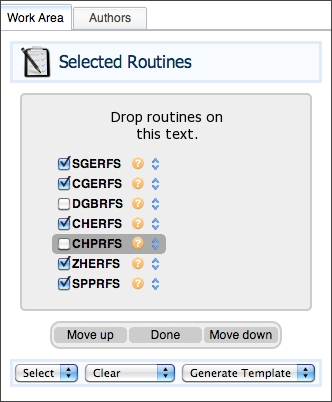
\includegraphics[width=3.5in]{figs/routineordering}
  \caption[Reordering routines]
   {Reordering selected routines in the Lighthouse work area.}
\end{figure}

\noindent  In Fall 2012, I took the numerical linear algebra class with Dr. Elizabeth Jessup in order to learn more about dense and sparse systems of linear equations, various algorithms for solving them, methods for solving eigenvalue problems, preconditioning and various other important topics in numerical linear algebra. In October, I started learning about PETSc and how to write programs using the library it provides. On November 2, I presented a poster about Lighthouse at the Rocky Mountain Celebration of Women in Computing Conference in Fort Collins, Colorado. On December 17, I proposed to add PETSc linear solvers to Lighthouse and write my Masters thesis about it.

\begin{figure}[h!]\label{lighthousePoster}
  \centering
  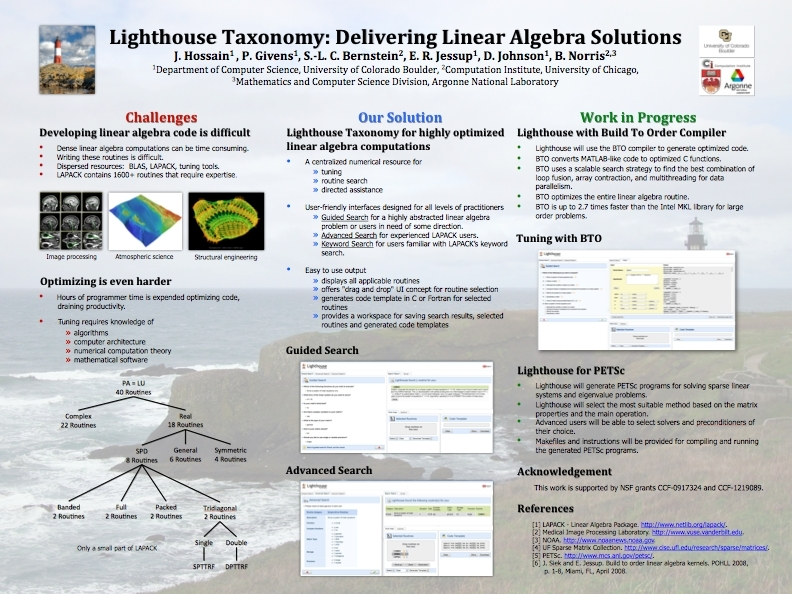
\includegraphics[width=6.5in]{figs/lighthousePoster}
  \caption[Lighthouse poster]
   {The Lighthouse poster presented at SIAM 2013 Computational Science and Engineeing Conference.}
\end{figure}


\noindent I continued learning and experimenting with PETSc and various iterative solvers. I also spent some time trying to learn how to use a matrix analysis module called AnaMod. On February 27, I attended the 2013 SIAM Conference on Computational Science and Engineering in Boston, Massachusetts where undergraduate research assistant Paul Givens and I presented an updated version of the Lighthouse poster. Figure 3.11 shows a screenshot of the poster we presented. Next, I began the process of integrating PETSc into Lighthouse, which is the main topic of this thesis (discussed in more detail in Chapter 4).